\documentclass[UTF8,fontset=fandol,11pt]{ctexart}
\usepackage[a4paper,margin=24mm,headheight=15pt]{geometry}
\usepackage{amsmath,amssymb,amsthm,mathtools,bm}
\usepackage{enumitem,booktabs,longtable,array,pdfpages,fancyhdr,xcolor}
\usepackage[colorlinks=true,linkcolor=blue!45!black,urlcolor=blue!45!black]{hyperref}
\allowdisplaybreaks[2]
\setlength{\parindent}{2em}
\setlength{\parskip}{3pt}
\setlength{\emergencystretch}{3em}
\setlist{nosep,topsep=3pt}
\pagestyle{fancy}\fancyhf{}\fancyhead[L]{\small 分析学讲义习题解答}\fancyhead[R]{\small 第38--57讲}\fancyfoot[C]{\thepage}
\newcommand{\R}{\mathbb R}\newcommand{\C}{\mathbb C}\newcommand{\N}{\mathbb N}\newcommand{\Z}{\mathbb Z}\newcommand{\Q}{\mathbb Q}\newcommand{\T}{\mathbb T}
\newcommand{\dd}{\,\mathrm d}\newcommand{\eps}{\varepsilon}\newcommand{\ind}{\mathbf1}
\newcommand{\norm}[1]{\left\lVert#1\right\rVert}\newcommand{\abs}[1]{\left|#1\right|}\newcommand{\ip}[2]{\left\langle#1,#2\right\rangle}
\DeclareMathOperator{\supp}{supp}\DeclareMathOperator{\rank}{rank}\DeclareMathOperator{\Span}{Span}\DeclareMathOperator{\diag}{diag}\DeclareMathOperator{\Res}{Res}\DeclareMathOperator{\Ext}{Ext}
\newcommand{\problem}[2]{\subsection*{#1}\addcontentsline{toc}{subsection}{#1}\noindent\textbf{题干。}#2\par\smallskip\noindent\textbf{解答。}}
\newcommand{\fix}[1]{\par\noindent\textcolor{red!55!black}{\textbf{原文核对与修正。}#1}\par}
\newcommand{\skipnote}[1]{\par\noindent\textbf{依约不解的计算题。}#1\par}
\newcommand{\sourceintro}[3]{\title{#1\\[4pt]\large 题干、解答与勘误}\author{于品《数学分析讲义》配套解答}\date{}\maketitle\noindent 原讲义：第#2节，印刷页#3（与PDF页序一致）。题干按数学内容重排；完整原题页附于文末，含未解的传统计算题，供逐字核对。原文中的作业提交说明及引文不作为本项目的工作指令。\par 本文中的“正函数”均按非负函数理解。复内积约定对第一个变量线性。}
\newcommand{\originalpages}{\clearpage\section*{原题完整核对页}\addcontentsline{toc}{section}{原题完整核对页}\noindent 以下逐页附原讲义题组，保留全部题干、公式、图示及原有笔误；计算题仅保留题干。\clearpage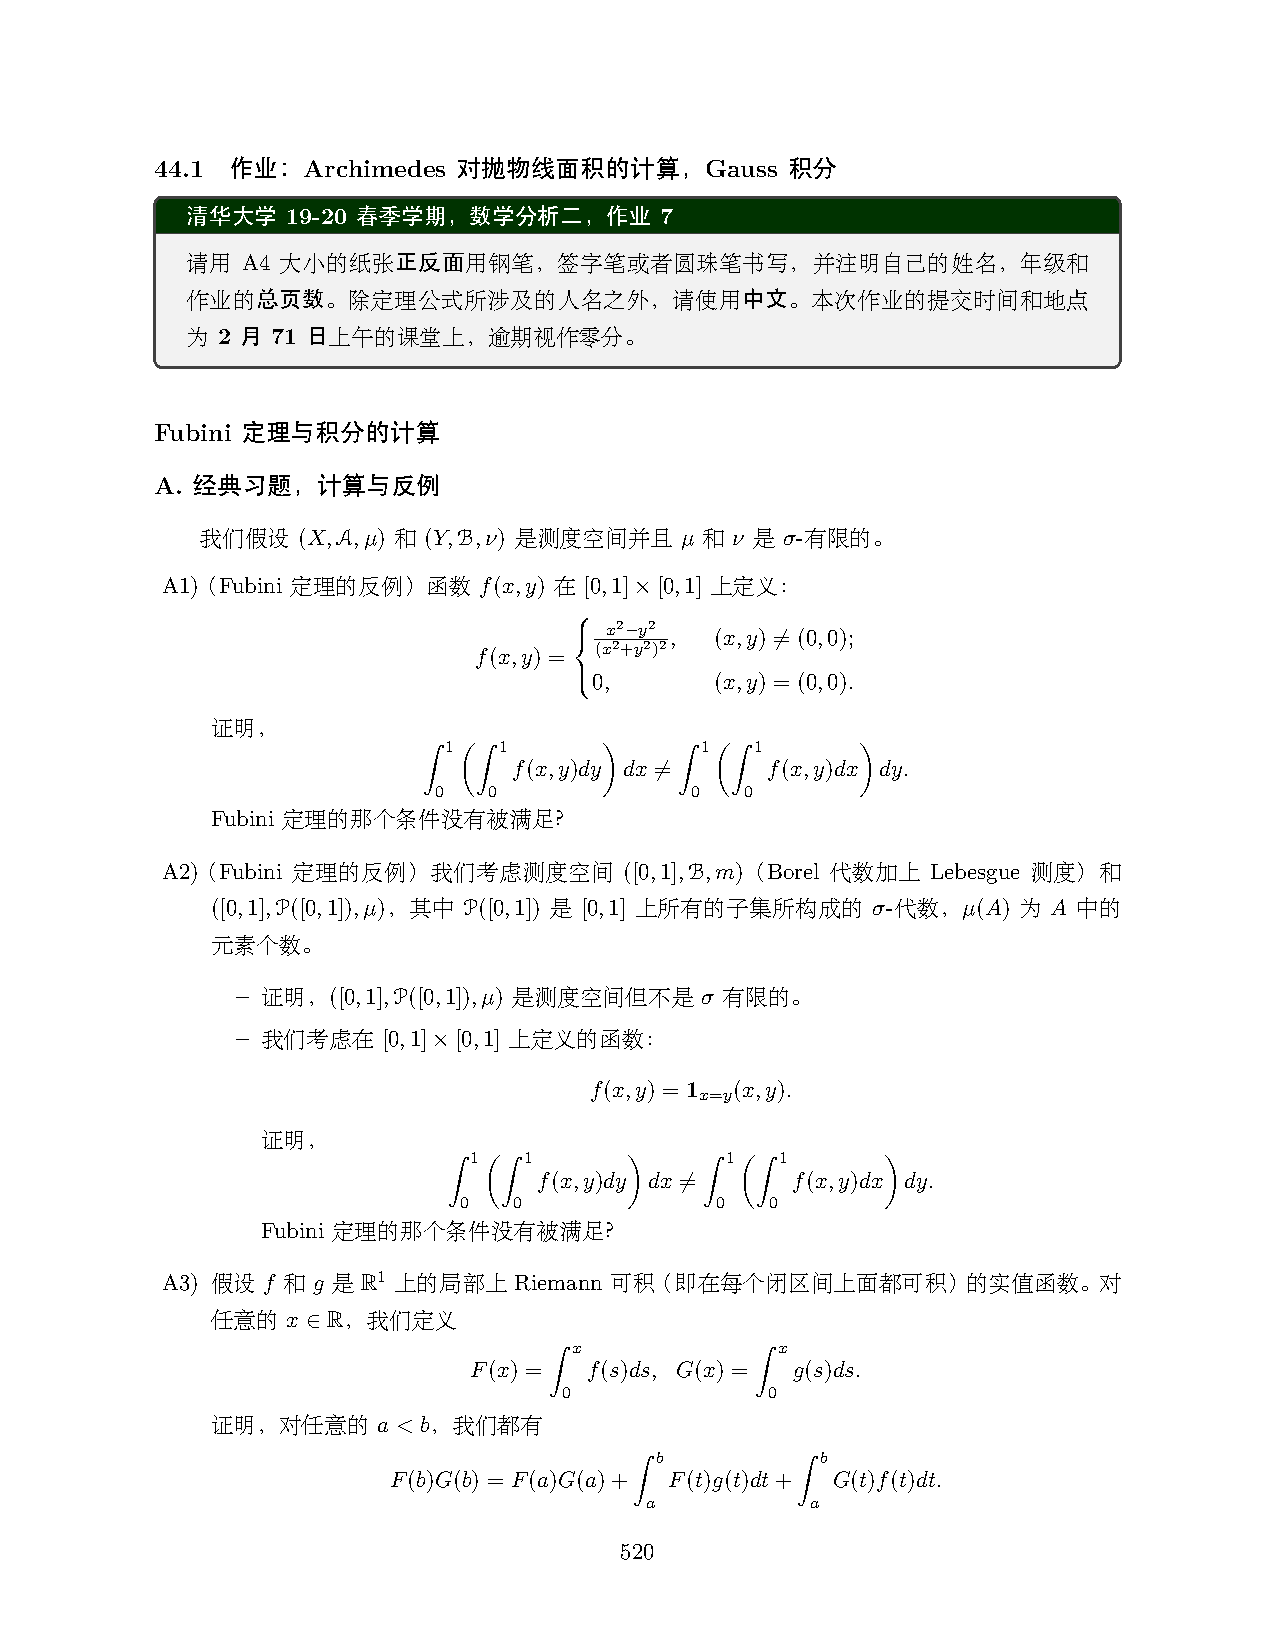
\includepdf[pages=-,pagecommand={\thispagestyle{empty}},scale=.94]{original.pdf}}

\begin{document}
\sourceintro{44.1 作业：Fubini定理、反例与抛物线}{44.1}{520--523}
\section*{所用知识}
第38--44讲：$\sigma$-有限乘积测度、Tonelli与Fubini定理；此前的隐函数定理和一元微积分。反例中的积分计算是展示定理条件必不可少的部分，保留。
\problem{A1}{在$[0,1]^2$令$f(x,y)=(x^2-y^2)/(x^2+y^2)^2$（原点置零）。证明两种累次积分不相等，并指出Fubini哪个条件不满足。}
对$x>0$，$f=\partial_y[y/(x^2+y^2)]$，所以$\int_0^1f(x,y)\dd y=1/(1+x^2)$；对$y>0$，$f=-\partial_x[x/(x^2+y^2)]$，所以$\int_0^1f(x,y)\dd x=-1/(1+y^2)$。两累次积分分别为$\pi/4,-\pi/4$。坐标轴上的异常截面不影响外积分，但原点附近在角度$0\le\theta\le\pi/6$的扇形上有$|f|\ge1/(2r^2)$，故$\int|f|\ge\frac12\int_0^1r^{-1}\dd r\int_0^{\pi/6}\dd\theta=\infty$。不满足绝对可积性。
\problem{A2}{第一因子为$([0,1],\mathcal B,m)$，第二因子为$([0,1],\mathcal P,\mu)$、$\mu$为计数测度。证明后者不是$\sigma$-有限；对$f(x,y)=\ind_{\{x=y\}}$，证明累次积分不同并解释。}
有限计数测度集合是有限集，可数个有限集不能覆盖不可数的$[0,1]$。按$y$用计数测度积分，每个$x$的截面质量为$1$，外积分为$1$；按$x$用Lebesgue测度积分，每个$y$的截面质量为$0$，外积分为$0$。对角线属于$\mathcal B\otimes\mathcal B\subset\mathcal B\otimes\mathcal P$，所以可测性没有问题；缺失的是第二因子的$\sigma$-有限性。
\problem{A3}{$f,g$局部Riemann可积，$F(x)=\int_0^xf(s)\dd s$、$G(x)=\int_0^xg(s)\dd s$。证明$F(b)G(b)=F(a)G(a)+\int_a^bF(t)g(t)\dd t+\int_a^bG(t)f(t)\dd t$。}
在$[a,b]$上写$F(t)=F(a)+\int_a^tf$、$G(t)=G(a)+\int_a^tg$。展开右端，两个三角形上的双重积分之和等于$\int_a^bf\int_a^bg$；对角线零测，且局部有界保证绝对可积。展开$F(b)G(b)$得到同一表达式。这避免了预先调用绝对连续函数的乘积法则。
\problem{A4}{原题给出$\sigma$-有限测度空间$(X,\mathcal A,\mu),(Y,\mathcal B,\nu)$，要求：(1)$D_\mu=\{x:\mu(\{x\})>0\}$可数；(2)$\Delta=\{(x,y)\in\R\times\R:x=y\}\subset X\times Y$可测；(3)$(\mu\otimes\nu)(\Delta)=\sum_{x\in D_\mu}\mu(\{x\})\nu(\{x\})$。}
\fix{一般空间中单点未必可测，也没有$X,Y\subset\R$。按题目中的对角线记法，补充$X=Y=\R$及两边均为Borel测度（或其完备化）。若仅假设任意可测空间，第(2)问甚至无法这样表述。}
取$\R=\bigcup_jE_j$、$\mu(E_j)<\infty$。每个$E_j$中质量至少$1/k$的点有限，故$D_\mu$可数。对角线为闭集，属于乘积Borel代数。Tonelli给出
\[(\mu\otimes\nu)(\Delta)=\int\mu(\{y\})\dd\nu(y)=\sum_{x\in D_\mu}\mu(\{x\})\nu(\{x\}).\]
因为$\sigma$-有限性使单点质量有限，乘积中没有$0\cdot\infty$歧义。
\problem{A5}{设$\Gamma=\{y=-cx^2\}$、$c>0$，$A,B$为其上不同两点。(1)证明$\Gamma$为光滑一维子流形且存在唯一$C$使切线平行$AB$；(2)过$C$的竖直线通过$AB$中点；(3)证明弓形面积是$\triangle ABC$面积的$4/3$。}
令$A=(a,-ca^2),B=(b,-cb^2)$，$a<b$。函数$y+cx^2$的梯度第二分量为$1$，零点集光滑。弦斜率为$-c(a+b)$，切线斜率$-2cx$，所以唯一$C$的横坐标为$(a+b)/2$，这也是弦中点横坐标。弦直线与抛物线之间的高度为$c(x-a)(b-x)$，其面积为$c(b-a)^3/6$。以$AB$的水平投影长度$b-a$和$C$到弦的竖直高度$c(b-a)^2/4$计算行列式，三角形面积为$c(b-a)^3/8$，比值$4/3$。这道历史定理的证明保留，未扩展成一般面积计算练习。
\skipnote{A6的四项Gauss积分、B1--B12、C1--C8的具体多重积分及D1--D3的具体面积体积计算不解。其完整题干保留于附录。}
\problem{A7*}{$f:\R^n\to\R$为Borel函数。证明除某个零测集$N\subset\R$外，对每个$y\notin N$，$m_n(\{x:f(x)=y\})=0$。}
各水平集两两不交。对每个整数$R,k\ge1$，在有限测度立方体$[-R,R]^n$内测度至少$1/k$的水平集至多$k(2R)^n$个。所有具有正测度的水平集都在某个这样的有限清单中出现，故其水平值集合至多可数，因而是$\R$的零测集。
\originalpages
\end{document}
